\documentclass[12pt]{article}
\usepackage[margin=1in]{geometry} 
\usepackage[utf8]{inputenc}
\usepackage[T1]{fontenc}
\usepackage{amsmath}
\usepackage{amsfonts}
\usepackage{amssymb}
\usepackage[version=4]{mhchem}
\usepackage{parskip}
\usepackage{booktabs}
\usepackage{stmaryrd}
\usepackage[margin=1in]{geometry} 
\usepackage{amsthm, graphicx, multicol, array}
 
\begin{document}
\title{Midterm Exam}
\author{Nicolas Moreno \\
ECON: 880}
\maketitle

\section{Baseline}

\begin{itemize}
    \item RA non-stochastic growth: $\rightarrow$ Ball park for Aggregate Capital.
\end{itemize}
$\rightarrow H H$ Preferences: $\sum_{t=0}^{\infty} \beta^{t} \ln \left(C_{t}\right)$ w/ $\beta=0.99$\\
$\rightarrow$ Technology: $Y_{t}=K_{t}^{\alpha} L_{t}^{1-\alpha}$\\
$\rightarrow$ Social Planner's:

$$
\begin{aligned}
\text { s.t. } &  \quad C_{t}+K_{t+1} \leq K_{t}^{\alpha} L_{t}^{1-\alpha} + (1-\delta) K_{t} \\
& L_{t}=\bar{e} \pi l
\end{aligned}
$$
\begin{itemize}
\item[$\rightarrow$] Given there is no labor disutility, $l=1 \quad \forall i$. 
\item[$\rightarrow$] By LNS of the utility function we know the resource constraint holds with equality and so:
\end{itemize}

\begin{itemize}
  \item We solve the unconstrained version of the problem: 
  \\
  F.O.C:
  \\
  $\left[K_{t+1}\right]:-\frac{\beta^{t}}{C_{t}}+\frac{\beta^{t+1}}{C_{t+1}}\left(\alpha \frac{Y_{t+1}}{K_{t+1}}+ 1-\delta\right)=0$\\
$\implies$ Euler Eqn.: $\frac{c_{t+1}}{C_{t}}=\beta\left(\alpha \frac{Y_{t+1}}{K_{t+1}} + 1-\delta\right)$
  \item Now, in SS without technological growth:
\end{itemize}

$$
\begin{aligned}
& c_{t+1}=c_{t}=\bar{c} ; y_{t}=\bar{y} ; k_{t}=k_{t+1}=\bar{k} \\
& \implies 1=\beta\left(\alpha \frac{\bar{y}}{\bar{k}}+1-\delta\right) \\
& \Leftrightarrow\left(\frac{1}{\beta}+\delta - 1\right)=\alpha \bar{k}^{\alpha-1}(\bar{e} \pi)^{1-\alpha} \\
& \Leftrightarrow \bar{k}=\left(\frac{1-\beta+\beta \delta}{\alpha \beta}\right)^{\frac{1}{\alpha-1}} \bar{e} \pi
\end{aligned}
$$

\begin{itemize}
  \item If we plug in parameter values in this analytical expression:
\end{itemize}

$$
\begin{aligned}
& \bar{K}=\left(\frac{1-(0.99)+(0.99)(0.025)}{(0.36)(0.99)}\right)^{-\frac{1}{0.64}}(0.3271)(0.93) \\
& \bar{K}= 11.556
\end{aligned}
$$

\section{Aiyagari Steady State}
As can be seen in the graph below, the steady state capital of the representative agent model (11.556) is lower than in the Aiyagari model (12.483). This result is consistent with greater precautionary saving by households, which comes from a utility function (log) that features constant relative risk aversion. Since agents prefer smooth consumption paths, when they face idiosyncratic shocks their savings increase and thus, they build up higher capital stocks that act as buffers against uncertainty. \\
\begin{figure}[h!]
    \centering
    \vspace{1cm}
    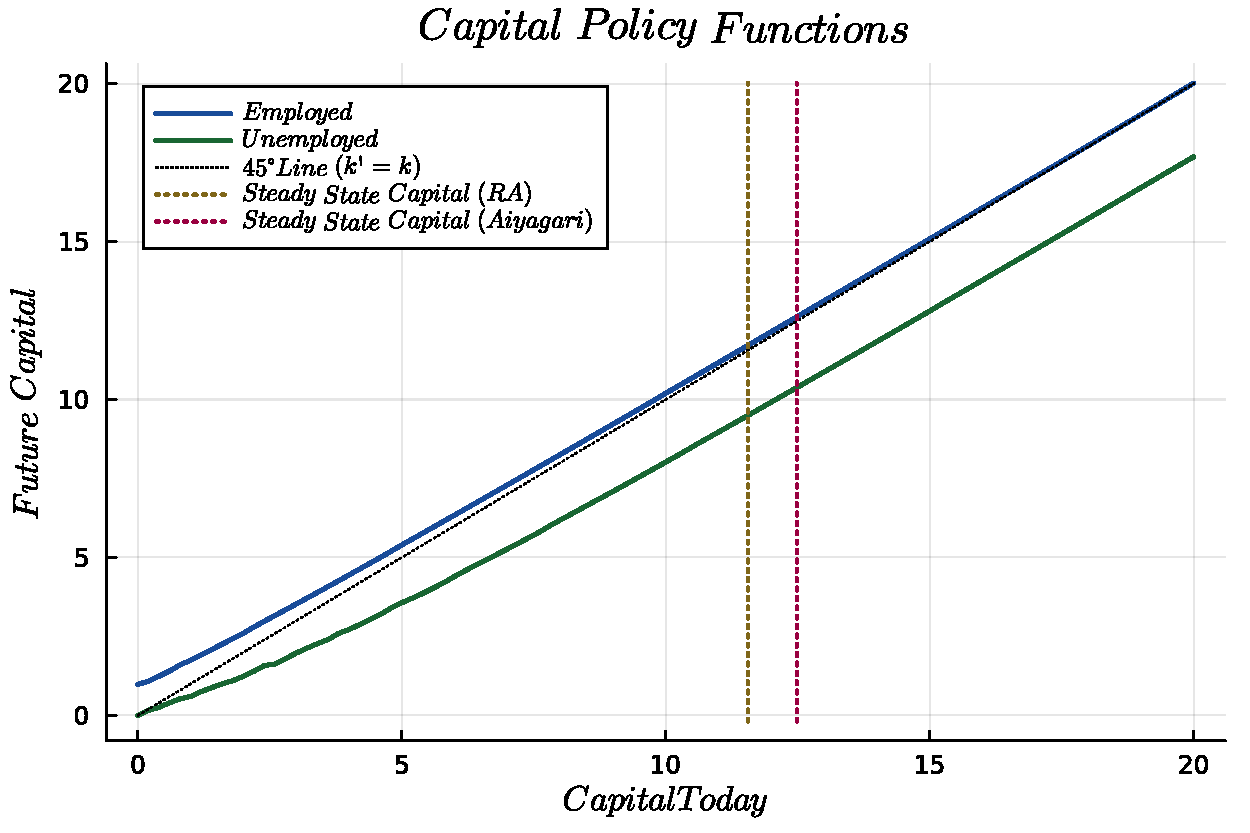
\includegraphics[scale=0.5]{Computational/Midterm/K_Policy_Func.pdf}
\end{figure}

The graph also shows how policy functions differ by employment status. Unemployed households cannot afford to save at the same rate of employed ones, even for high initial capital holdings. Hence, the policy function of the employed is always above that of the unemployed and, as expected, intersects the $45°$ degree line at a level above the steady state level, whereas that of the unemployed intersects it to the at a level below.
\newpage
\section{Krusell-Smith}
Following the algorithm suggested in both the handout and the pseudocode file, my code converged in 3 iterations. The results obtained for the law of motion of capital are summarized in Table \ref{tab:parameter_estimations}. We can see that the intercept is higher than the initial guess, both in bad and good times.
\begin{table}[h!]
\centering
\begin{tabular}{lcc}
\toprule
\textbf{Estimate} & \textbf{Initial Guess} & \textbf{Final Estimation} \\
\midrule
\(a_0\) & 0.095 & 0.1342 \\
\(a_1\) & 0.599 & 0.9483 \\
\(b_0\) & 0.085 & 0.1188 \\
\(b_1\) & 0.599 & 0.9507 \\
\(R^2\) & 0.0   & 1.0   \\
\bottomrule
\end{tabular}
\caption{Initial Guess and Final Estimation of Parameters}
\label{tab:parameter_estimations}
\end{table}
Here I also plot the behavior of aggregate capital in the last simulation performed to update the regression parameters, and we can see that the mean is a bit below the initial steady state level.
\begin{figure}[h!]
    \centering
    \vspace{1cm}
    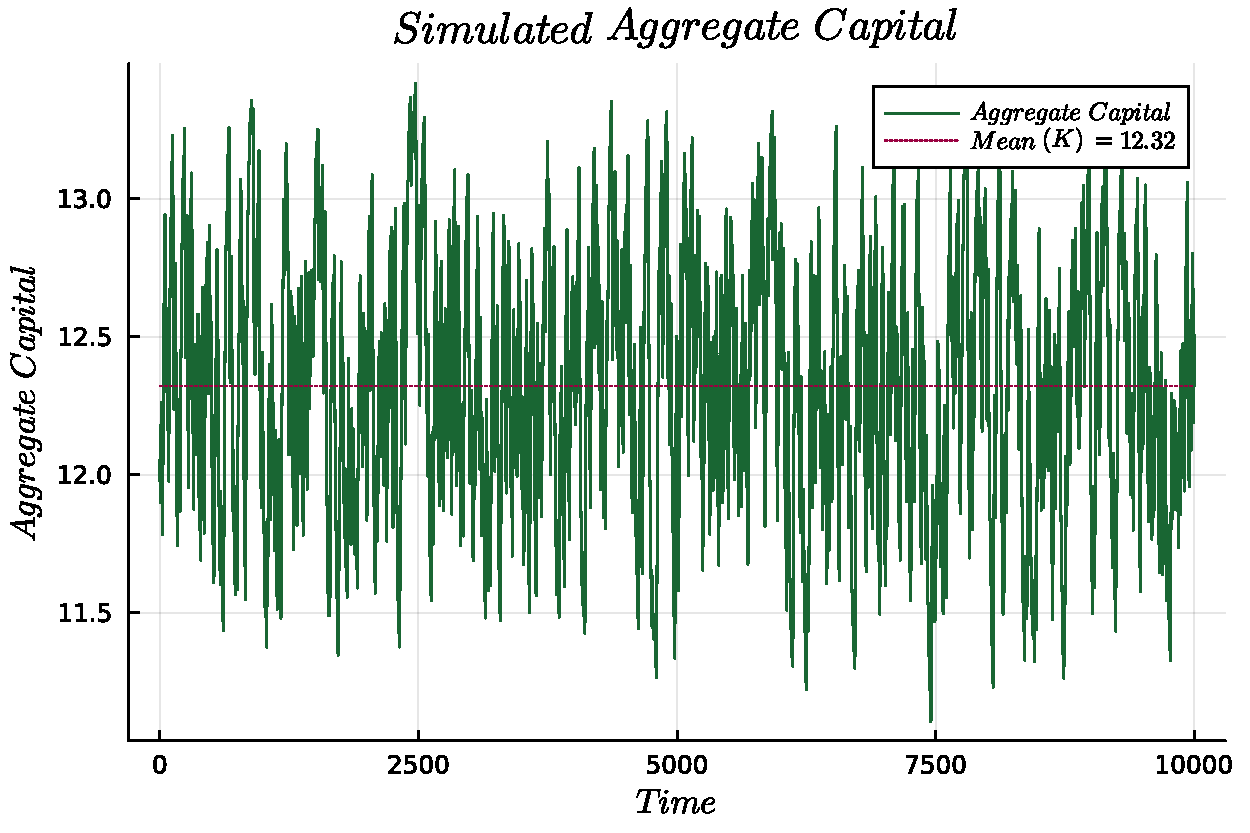
\includegraphics[scale=0.5]{Computational/Midterm/Simulated_K.pdf}
\end{figure}


\end{document}





